\chapter{Backpropagation}

\section*{Introduction}

\paragraph*{Motivation} In this section we will develop expertise with an intuitive understanding of backpropagation, which is a way of computing gradients of expressions through recursive application of \textbf{chain rule}. Understanding of this process and its subtleties is critical for you to understand, and effectively develop, design and debug Neural Networks.

\paragraph*{Problem statement} The core problem studied in this section is as follows: We are given some function $f(x)$ where $x$ is a vector of inputs and we are interested in computing the gradient of $f$ at $x$ (i.e. $\nabla f(x)$ ).

\paragraph*{Motivation} Recall that the primary reason we are interested in this problem is that in the specific case of Neural Networks, $f$ will correspond to the loss function ( $L$ ) and the inputs $x$ will consist of the training data and the neural network weights. For example, the loss could be the SVM loss function and the inputs are both the training data $(x_i,y_i), i=1 \ldots N$ and the weights and biases $W,b$. Note that (as is usually the case in Machine Learning) we think of the training data as given and fixed, and of the weights as variables we have control over. Hence, even though we can easily use backpropagation to compute the gradient on the input examples $x_i$, in practice we usually only compute the gradient for the parameters (e.g. $W,b$) so that we can use it to perform a parameter update. However, as we will see later in the class the gradient on xixi can still be useful sometimes, for example for purposes of visualization and interpreting what the Neural Network might be doing.

\section*{Simple expressions and interpretation of the gradient}

Lets start simple so that we can develop the notation and conventions for more complex expressions. Consider a simple multiplication function of two numbers $f(x,y)=xy$. It is a matter of simple calculus to derive the partial derivative for either input:

\begin{equation}
f(x,y) = x y \hspace{0.5in} \rightarrow \hspace{0.5in} \frac{\partial f}{\partial x} = y \hspace{0.5in} \frac{\partial f}{\partial y} = x
\end{equation}

\paragraph*{Interpretation} Keep in mind what the derivatives tell you: They indicate the rate of change of a function with respect to that variable surrounding an infinitesimally small region near a particular point:
\begin{equation}
\frac{df(x)}{dx} = \lim_{h\ \to 0} \frac{f(x + h) - f(x)}{h}
\end{equation}
A technical note is that the division sign on the left-hand sign is, unlike the division sign on the right-hand sign, not a division. Instead, this notation indicates that the operator $\frac{d}{dx}$ is being applied to the function $f$, and returns a different function (the derivative). A nice way to think about the expression above is that when $h$ is very small, then the function is well-approximated by a straight line, and the derivative is its slope. In other words, the derivative on each variable tells you the sensitivity of the whole expression on its value. For example, if $x=4,y=-3$ then $f(x,y)=-12$ and the derivative on $x$ $\frac{\partial f}{\partial x} = -3$. This tells us that if we were to increase the value of this variable by a tiny amount, the effect on the whole expression would be to decrease it (due to the negative sign), and by three times that amount. This can be seen by rearranging the above equation ( $f(x + h) = f(x) + h \frac{df(x)}{dx}$ ). Analogously, since $\frac{\partial f}{\partial y} = 4$, we expect that increasing the value of $y$ by some very small amount $h$ would also increase the output of the function (due to the positive sign), and by $4h$.

The derivative on each variable tells you the sensitivity of the whole expression on its value.

As mentioned, the gradient $\nabla f$ is the vector of partial derivatives, so we have that $\nabla f = [\frac{\partial f}{\partial x}, \frac{\partial f}{\partial y}] = [y, x]$. Even though the gradient is technically a vector, we will often use terms such as ``the gradient on x" instead of the technically correct phrase ``the partial derivative on x" for simplicity.

We can also derive the derivatives for the addition operation:

\begin{equation}
f(x,y) = x + y \hspace{0.5in} \rightarrow \hspace{0.5in} \frac{\partial f}{\partial x} = 1 \hspace{0.5in} \frac{\partial f}{\partial y} = 1
\end{equation}

that is, the derivative on both $x,y$ is one regardless of what the values of $x,y$ are. This makes sense, since increasing either $x,y$ would increase the output of $f$, and the rate of that increase would be independent of what the actual values of $x,y$ are (unlike the case of multiplication above). The last function we’ll use quite a bit in the class is the max operation:

\begin{equation}
f(x,y) = \max(x, y) \hspace{0.5in} \rightarrow \hspace{0.5in} \frac{\partial f}{\partial x} = (x >= y) \hspace{0.5in} \frac{\partial f}{\partial y} = (y >= x)
\end{equation}

That is, the (sub)gradient is 1 on the input that was larger and 0 on the other input. Intuitively, if the inputs are $x=4,y=2$, then the max is 4, and the function is not sensitive to the setting of $y$. That is, if we were to increase it by a tiny amount $h$, the function would keep outputting 4, and therefore the gradient is zero: there is no effect. Of course, if we were to change $y$ by a large amount (e.g. larger than 2), then the value of $f$ would change, but the derivatives tell us nothing about the effect of such large changes on the inputs of a function; They are only informative for tiny, infinitesimally small changes on the inputs, as indicated by the $\lim_{h \rightarrow 0}$ in its definition.


\section*{Compound expressions with chain rule}

Lets now start to consider more complicated expressions that involve multiple composed functions, such as $f(x,y,z) = (x + y) z$. This expression is still simple enough to differentiate directly, but we’ll take a particular approach to it that will be helpful with understanding the intuition behind backpropagation. In particular, note that this expression can be broken down into two expressions: $q=x+y$ and $f=qz$. Moreover, we know how to compute the derivatives of both expressions separately, as seen in the previous section. $f$ is just multiplication of $q$ and $z$, so $\frac{\partial f}{\partial q} = z, \frac{\partial f}{\partial z} = q$ and $q$ is addition of $x$ and $y$ so $\frac{\partial q}{\partial x} = 1, \frac{\partial q}{\partial y} = 1$. However, we don’t necessarily care about the gradient on the intermediate value $q$ - the value of $\frac{\partial f}{\partial q}$ is not useful. Instead, we are ultimately interested in the gradient of $f$ with respect to its inputs $x,y,z$. The chain rule tells us that the correct way to ``chain” these gradient expressions together is through multiplication. For example, $\frac{\partial f}{\partial x} = \frac{\partial f}{\partial q} \frac{\partial q}{\partial x}$. In practice this is simply a multiplication of the two numbers that hold the two gradients. Lets see this with an example:

\begin{lstlisting}[frame=single]
# set some inputs
x = -2; y = 5; z = -4

# perform the forward pass
q = x + y # q becomes 3
f = q * z # f becomes -12

# perform the backward pass (backpropagation) in reverse order:
# first backprop through f = q * z
dfdz = q # df/dz = q, so gradient on z becomes 3
dfdq = z # df/dq = z, so gradient on q becomes -4
# now backprop through q = x + y
dfdx = 1.0 * dfdq # dq/dx = 1. And the multiplication here is the chain rule!
dfdy = 1.0 * dfdq # dq/dy = 1
\end{lstlisting}

At the end we are left with the gradient in the variables \texttt{[dfdx,dfdy,dfdz]}, which tell us the sensitivity of the variables \texttt{x,y,z} on \texttt{f}. This is the simplest example of backpropagation. Going forward, we will want to use a more concise notation so that we don’t have to keep writing the \texttt{df} part. That is, for example instead of \texttt{dfdq} we would simply write \texttt{dq}, and always assume that the gradient is with respect to the final output.

\begin{figure}[h]
  \centering
  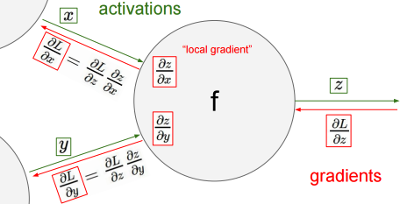
\includegraphics[width=0.5\textwidth]{Images/backprop/1.png}
  \caption{Neuron backprop}
\end{figure}

This computation can also be nicely visualized with a circuit diagram in figure \ref{fig:backdiag1}. The real-valued ``circuit" shows the visual representation of the computation. The forward pass computes values from inputs to output (shown in green). The backward pass then performs backpropagation which starts at the end and recursively applies the chain rule to compute the gradients (shown in red) all the way to the inputs of the circuit. The gradients can be thought of as flowing backwards through the circuit.

\begin{figure}[h]
  \centering
  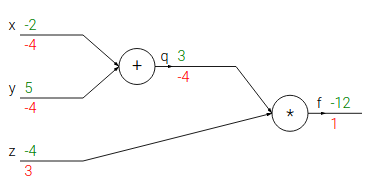
\includegraphics[width=0.5\textwidth]{Images/backprop/2.png}
  \caption{Neuron backprop diagram}
   \label{fig:backdiag1}
\end{figure}

\section*{Intuitive understanding of backpropagation}

Notice that backpropagation is a beautifully local process. Every gate in a circuit diagram gets some inputs and can right away compute two things: 1. its output value and 2. the local gradient of its inputs with respect to its output value. Notice that the gates can do this completely independently without being aware of any of the details of the full circuit that they are embedded in. However, once the forward pass is over, during backpropagation the gate will eventually learn about the gradient of its output value on the final output of the entire circuit. Chain rule says that the gate should take that gradient and multiply it into every gradient it normally computes for all of its inputs.

This extra multiplication (for each input) due to the chain rule can turn a single and relatively useless gate into a cog in a complex circuit such as an entire neural network.

Lets get an intuition for how this works by referring again to the example. The add gate received inputs [-2, 5] and computed output 3. Since the gate is computing the addition operation, its local gradient for both of its inputs is +1. The rest of the circuit computed the final value, which is -12. During the backward pass in which the chain rule is applied recursively backwards through the circuit, the add gate (which is an input to the multiply gate) learns that the gradient for its output was -4. If we anthropomorphize the circuit as wanting to output a higher value (which can help with intuition), then we can think of the circuit as “wanting” the output of the add gate to be lower (due to negative sign), and with a force of 4. To continue the recurrence and to chain the gradient, the add gate takes that gradient and multiplies it to all of the local gradients for its inputs (making the gradient on both $x$ and $y$ 1 * -4 = -4). Notice that this has the desired effect: If $x,y$ were to decrease (responding to their negative gradient) then the add gate’s output would decrease, which in turn makes the multiply gate’s output increase.

Backpropagation can thus be thought of as gates communicating to each other (through the gradient signal) whether they want their outputs to increase or decrease (and how strongly), so as to make the final output value higher.


\section*{Modularity: Sigmoid example}

The gates we introduced above are relatively arbitrary. Any kind of differentiable function can act as a gate, and we can group multiple gates into a single gate, or decompose a function into multiple gates whenever it is convenient. Lets look at another expression that illustrates this point:
\begin{equation}
f(w,x) = \frac{1}{1+e^{-(w_0x_0 + w_1x_1 + w_2)}}
\end{equation}
as we will see later in the class, this expression describes a 2-dimensional neuron (with inputs $x$ and weights $w$) that uses the sigmoid activation function. But for now lets think of this very simply as just a function from inputs w,x to a single number. The function is made up of multiple gates. In addition to the ones described already above (add, mul, max), there are four more:

\begin{equation}
f(x) = \frac{1}{x} 
 \rightarrow 
\frac{df}{dx} = -1/x^2 ,
\\\\
\hspace{0.1in}f_c(x) = c + x
 \rightarrow  
\frac{df}{dx} = 1,
\\\\
\hspace{0.1in}f(x) = e^x
 \rightarrow 
\frac{df}{dx} = e^x,
\\\\
\hspace{0.1in}f_a(x) = ax
 \rightarrow  
\frac{df}{dx} = a
\end{equation}

Where the functions $f_c,f_a$ translate the input by a constant of $c$ and scale the input by a constant of $a$, respectively. These are technically special cases of addition and multiplication, but we introduce them as (new) unary gates here since we do need the gradients for the constants. $c,a$. The full circuit then looks as follows:

\begin{figure}[h]
  \centering
  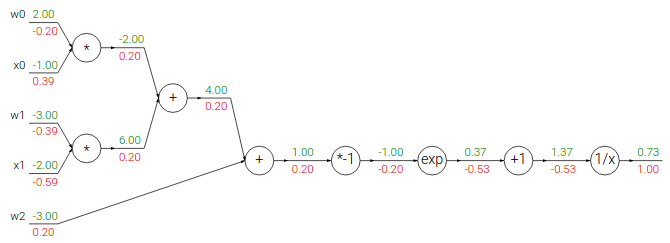
\includegraphics[width=0.7\textwidth]{Images/backprop/3.png}
  \caption{Example circuit for a 2D neuron with a sigmoid activation function. The inputs are $[x0,x1]$ and the (learnable) weights of the neuron are $[w0,w1,w2]$. As we will see later, the neuron computes a dot product with the input and then its activation is softly squashed by the sigmoid function to be in range from 0 to 1.}
\end{figure}

In the example above, we see a long chain of function applications that operates on the result of the dot product between $w,x$. The function that these operations implement is called the sigmoid function $\sigma(x)$. It turns out that the derivative of the sigmoid function with respect to its input simplifies if you perform the derivation (after a fun tricky part where we add and subtract a 1 in the numerator):

\begin{equation}
\sigma(x) = \frac{1}{1+e^{-x}} \\\\
\rightarrow \frac{d\sigma(x)}{dx} = \frac{e^{-x}}{(1+e^{-x})^2} = \left( \frac{1 + e^{-x} - 1}{1 + e^{-x}} \right) \left( \frac{1}{1+e^{-x}} \right) 
= \left( 1 - \sigma(x) \right) \sigma(x)
\end{equation}

As we see, the gradient turns out to simplify and becomes surprisingly simple. For example, the sigmoid expression receives the input 1.0 and computes the output 0.73 during the forward pass. The derivation above shows that the local gradient would simply be (1 - 0.73) * 0.73 ~= 0.2, as the circuit computed before (see the image above), except this way it would be done with a single, simple and efficient expression (and with less numerical issues). Therefore, in any real practical application it would be very useful to group these operations into a single gate. Lets see the backprop for this neuron in code:

\begin{lstlisting}[frame=single]
w = [2,-3,-3] # assume some random weights and data
x = [-1, -2]

# forward pass
dot = w[0]*x[0] + w[1]*x[1] + w[2]
f = 1.0 / (1 + math.exp(-dot)) # sigmoid function

# backward pass through the neuron (backpropagation)
ddot = (1 - f) * f # gradient on dot variable, using the sigmoid gradient derivation
dx = [w[0] * ddot, w[1] * ddot] # backprop into x
dw = [x[0] * ddot, x[1] * ddot, 1.0 * ddot] # backprop into w
# we're done! we have the gradients on the inputs to the circuit
\end{lstlisting}

\paragraph*{Implementation protip} staged backpropagation. As shown in the code above, in practice it is always helpful to break down the forward pass into stages that are easily backpropped through. For example here we created an intermediate variable \texttt{dot} which holds the output of the dot product between \texttt{w} and \texttt{x}. During backward pass we then successively compute (in reverse order) the corresponding variables (e.g. \texttt{ddot}, and ultimately \texttt{dw}, \texttt{dx}) that hold the gradients of those variables.

The point of this section is that the details of how the backpropagation is performed, and which parts of the forward function we think of as gates, is a matter of convenience. It helps to be aware of which parts of the expression have easy local gradients, so that they can be chained together with the least amount of code and effort.


\section*{Backprop in practice: Staged computation}

Lets see this with another example. Suppose that we have a function of the form:
\begin{equation}
f(x,y) = \frac{x + \sigma(y)}{\sigma(x) + (x+y)^2}
\end{equation}
To be clear, this function is completely useless and it’s not clear why you would ever want to compute its gradient, except for the fact that it is a good example of backpropagation in practice. It is very important to stress that if you were to launch into performing the differentiation with respect to either $x$ or $y$, you would end up with very large and complex expressions. However, it turns out that doing so is completely unnecessary because we don’t need to have an explicit function written down that evaluates the gradient. We only have to know how to compute it. Here is how we would structure the forward pass of such expression:

\begin{lstlisting}[frame=single]
x = 3 # example values
y = -4

# forward pass
sigy = 1.0 / (1 + math.exp(-y)) # sigmoid in numerator   #(1)
num = x + sigy # numerator                               #(2)
sigx = 1.0 / (1 + math.exp(-x)) # sigmoid in denominator #(3)
xpy = x + y                                              #(4)
xpysqr = xpy**2                                          #(5)
den = sigx + xpysqr # denominator                        #(6)
invden = 1.0 / den                                       #(7)
f = num * invden # done!                                 #(8)
\end{lstlisting}

Phew, by the end of the expression we have computed the forward pass. Notice that we have structured the code in such way that it contains multiple intermediate variables, each of which are only simple expressions for which we already know the local gradients. Therefore, computing the backprop pass is easy: We’ll go backwards and for every variable along the way in the forward pass (\texttt{sigy, num, sigx, xpy, xpysqr, den, invden}) we will have the same variable, but one that begins with a \texttt{d}, which will hold the gradient of the output of the circuit with respect to that variable. Additionally, note that every single piece in our backprop will involve computing the local gradient of that expression, and chaining it with the gradient on that expression with a multiplication. For each row, we also highlight which part of the forward pass it refers to:

\begin{lstlisting}[frame=single]
# backprop f = num * invden
dnum = invden # gradient on numerator                             #(8)
dinvden = num                                                     #(8)
# backprop invden = 1.0 / den 
dden = (-1.0 / (den**2)) * dinvden                                #(7)
# backprop den = sigx + xpysqr
dsigx = (1) * dden                                                #(6)
dxpysqr = (1) * dden                                              #(6)
# backprop xpysqr = xpy**2
dxpy = (2 * xpy) * dxpysqr                                        #(5)
# backprop xpy = x + y
dx = (1) * dxpy                                                   #(4)
dy = (1) * dxpy                                                   #(4)
# backprop sigx = 1.0 / (1 + math.exp(-x))
dx += ((1 - sigx) * sigx) * dsigx # Notice += !! See notes below  #(3)
# backprop num = x + sigy
dx += (1) * dnum                                                  #(2)
dsigy = (1) * dnum                                                #(2)
# backprop sigy = 1.0 / (1 + math.exp(-y))
dy += ((1 - sigy) * sigy) * dsigy                                 #(1)
# done! phew
\end{lstlisting}

Notice a few things:

\paragraph*{Cache forward pass variables} To compute the backward pass it is very helpful to have some of the variables that were used in the forward pass. In practice you want to structure your code so that you cache these variables, and so that they are available during backpropagation. If this is too difficult, it is possible (but wasteful) to recompute them.

\paragraph*{Gradients add up at forks} The forward expression involves the variables $x,y$ multiple times, so when we perform backpropagation we must be careful to use \texttt{+=} instead of \texttt{=} to accumulate the gradient on these variables (otherwise we would overwrite it). This follows the multivariable chain rule in Calculus, which states that if a variable branches out to different parts of the circuit, then the gradients that flow back to it will add.


\section*{Patterns in backward flow}

It is interesting to note that in many cases the backward-flowing gradient can be interpreted on an intuitive level. For example, the three most commonly used gates in neural networks (add,mul,max), all have very simple interpretations in terms of how they act during backpropagation. Consider this example circuit:

\begin{figure}[h]
  \centering
  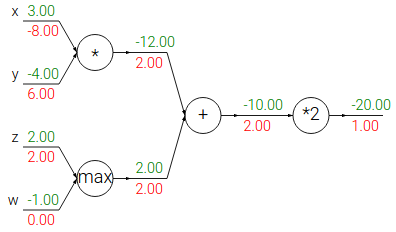
\includegraphics[width=0.4\textwidth]{Images/backprop/4.png}
  \caption{An example circuit demonstrating the intuition behind the operations that backpropagation performs during the backward pass in order to compute the gradients on the inputs. Sum operation distributes gradients equally to all its inputs. Max operation routes the gradient to the higher input. Multiply gate takes the input activations, swaps them and multiplies by its gradient.
}
\end{figure}

Looking at the diagram above as an example, we can see that:

\paragraph*{add gate} The add gate always takes the gradient on its output and distributes it equally to all of its inputs, regardless of what their values were during the forward pass. This follows from the fact that the local gradient for the add operation is simply +1.0, so the gradients on all inputs will exactly equal the gradients on the output because it will be multiplied by x1.0 (and remain unchanged). In the example circuit above, note that the + gate routed the gradient of 2.00 to both of its inputs, equally and unchanged.

\paragraph*{max gate} The max gate routes the gradient. Unlike the add gate which distributed the gradient unchanged to all its inputs, the max gate distributes the gradient (unchanged) to exactly one of its inputs (the input that had the highest value during the forward pass). This is because the local gradient for a max gate is 1.0 for the highest value, and 0.0 for all other values. In the example circuit above, the max operation routed the gradient of 2.00 to the z variable, which had a higher value than w, and the gradient on w remains zero.

\paragraph*{multiply gate} The multiply gate is a little less easy to interpret. Its local gradients are the input values (except switched), and this is multiplied by the gradient on its output during the chain rule. In the example above, the gradient on x is -8.00, which is -4.00 x 2.00.

Unintuitive effects and their consequences. Notice that if one of the inputs to the multiply gate is very small and the other is very big, then the multiply gate will do something slightly unintuitive: it will assign a relatively huge gradient to the small input and a tiny gradient to the large input. Note that in linear classifiers where the weights are dot producted $w^Tx_i$ (multiplied) with the inputs, this implies that the scale of the data has an effect on the magnitude of the gradient for the weights. For example, if you multiplied all input data examples $x_i$ by 1000 during preprocessing, then the gradient on the weights will be 1000 times larger, and you’d have to lower the learning rate by that factor to compensate. This is why preprocessing matters a lot, sometimes in subtle ways! And having intuitive understanding for how the gradients flow can help you debug some of these cases.


\section*{Gradients for vectorized operations}

The above sections were concerned with single variables, but all concepts extend in a straight-forward manner to matrix and vector operations. However, one must pay closer attention to dimensions and transpose operations.

\paragraph*{Matrix-Matrix multiply gradient} Possibly the most tricky operation is the matrix-matrix multiplication (which generalizes all matrix-vector and vector-vector) multiply operations:

\begin{lstlisting}[frame=single]
# forward pass
W = np.random.randn(5, 10)
X = np.random.randn(10, 3)
D = W.dot(X)

# now suppose we had the gradient on D from above in the circuit
dD = np.random.randn(*D.shape) # same shape as D
dW = dD.dot(X.T) #.T gives the transpose of the matrix
dX = W.T.dot(dD)
\end{lstlisting}

\textbf{Tip}: use dimension analysis! Note that you do not need to remember the expressions for \texttt{dW} and \texttt{dX} because they are easy to re-derive based on dimensions. For instance, we know that the gradient on the weights \texttt{dW} must be of the same size as \texttt{W} after it is computed, and that it must depend on matrix multiplication of \texttt{X} and \texttt{dD} (as is the case when both \texttt{X,W} are single numbers and not matrices). There is always exactly one way of achieving this so that the dimensions work out. For example, \texttt{X} is of size [10 x 3] and \texttt{dD} of size [5 x 3], so if we want \texttt{dW} and \texttt{W} has shape [5 x 10], then the only way of achieving this is with \texttt{dD.dot(X.T)}, as shown above.

\paragraph*{Work with small, explicit examples}. Some people may find it difficult at first to derive the gradient updates for some vectorized expressions. Our recommendation is to explicitly write out a minimal vectorized example, derive the gradient on paper and then generalize the pattern to its efficient, vectorized form.

Erik Learned-Miller has also written up a longer related document on taking matrix/vector derivatives which you might find helpful. Find it here.


\section*{Summary}
\begin{itemize}
\item We developed intuition for what the gradients mean, how they flow backwards in the circuit, and how they communicate which part of the circuit should increase or decrease and with what force to make the final output higher.
\item We discussed the importance of staged computation for practical implementations of backpropagation. You always want to break up your function into modules for which you can easily derive local gradients, and then chain them with chain rule. Crucially, you almost never want to write out these expressions on paper and differentiate them symbolically in full, because you never need an explicit mathematical equation for the gradient of the input variables. Hence, decompose your expressions into stages such that you can differentiate every stage independently (the stages will be matrix vector multiplies, or max operations, or sum operations, etc.) and then backprop through the variables one step at a time.
\end{itemize}

In the next section we will start to define Neural Networks, and backpropagation will allow us to efficiently compute the gradients on the connections of the neural network, with respect to a loss function. In other words, we’re now ready to train Neural Nets, and the most conceptually difficult part of this class is behind us! ConvNets will then be a small step away.